\documentclass[a4paper, 12pt]{article}

\usepackage{graphicx}
\usepackage{longtable}
\graphicspath{ {images/} }

\newcommand{\templates}{../../template}
\usepackage[a4paper, margin=2.5cm]{geometry}

\usepackage{enumitem}
\setlist[itemize]{noitemsep}
\setlist[enumerate]{noitemsep}

\let\oldpar\paragraph
\renewcommand{\paragraph}[1]{\oldpar{#1\\}\noindent}
\usepackage{graphicx}
\usepackage{hyperref}
\usepackage{makecell}

\newcommand{\settitolo}[1]{\newcommand{\titolo}{#1\\}}
\newcommand{\setprogetto}[1]{\newcommand{\progetto}{#1\\}}
\newcommand{\setcommittenti}[1]{\newcommand{\committenti}{#1\\}}
\newcommand{\setredattori}[1]{\newcommand{\redattori}{#1\\}}
\newcommand{\setrevisori}[1]{\newcommand{\revisori}{#1\\}}
\newcommand{\setresponsabili}[1]{\newcommand{\responsabili}{#1\\}}
\newcommand{\setversione}[1]{
	\ifdefined\versione\renewcommand{\versione}{#1\\}
	\else\newcommand{\versione}{#1\\}\fi
}
\newcommand{\setdestuso}[1]{\newcommand{\uso}{#1\\}}
\newcommand{\setdescrizione}[1]{\newcommand{\descrizione}{#1\\}}

\newcommand{\makefrontpage}{
	\begin{titlepage}
		\begin{center}

		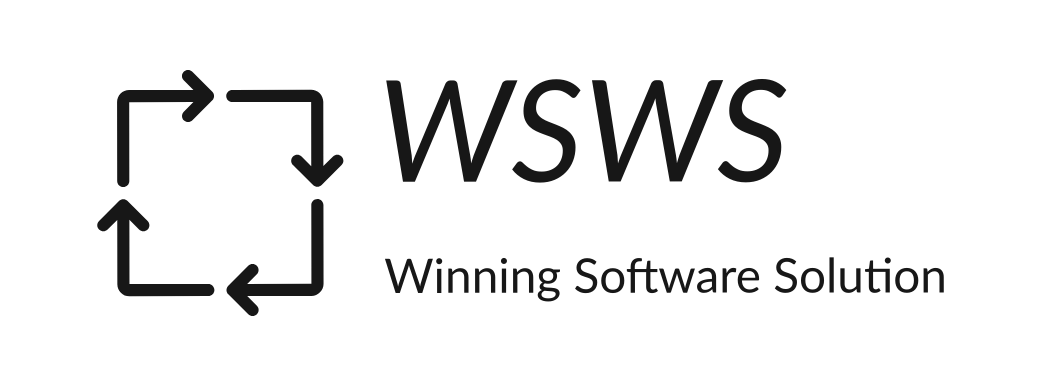
\includegraphics[width=0.4\textwidth]{../../template/WSWS-logos_transparent_crop}\\

		{\Large Winning Software Solution}\\[6pt]
		\href{mailto://winningsoftwaresolution@gmail.com}{winningsoftwaresolution@gmail.com}\\
		
		\ifdefined\progetto
		\vspace{1cm}
		{\Large\progetto}
		{\large\committenti}
		\else\fi
		
		\vspace{1.5cm}
		{\LARGE\titolo}
		
		\vfill
		
		\begin{tabular}{r | l}
		\multicolumn{2}{c}{\textit{Informazioni}}\\
		\hline
		
		\ifdefined\redattori
			\textit{Redattori} &
			\makecell[l]{\redattori}\\
		\else\fi
		\ifdefined\revisori
			\textit{Revisori} &
			\makecell[l]{\revisori}\\
		\else\fi
		\ifdefined\responsabili
			\textit{Respondabili} &
			\makecell[l]{\responsabili}\\
		\else\fi
		
		\ifdefined\versione
			\textit{Versione} & \versione
		\else\fi
		
		\textit{Uso} & \uso
		
		\end{tabular}
		
		\vspace{2cm}
		
		\ifdefined\descrizione
		Descrizione
		\vspace{6pt}
		\hrule
		\descrizione
		\else\fi
		\end{center}
	\end{titlepage}
}
\usepackage{hyperref}
\usepackage{array}
\usepackage{tabularx}

\def\vers#1-#2-#3-#4-#5\\{#1&#2&#3&#4&#5\\\hline}

\newcommand{\addversione}[5]{
	\ifdefined\versioni
		\let\old\versioni
		\renewcommand{\versioni}{#1&#2&#3&#4&#5\\\hline\old}
	\else
		\newcommand{\versioni}{#1&#2&#3&#4&#5\\\hline}
	\fi
}

\newcommand{\setversioni}[1]{\newcommand{\versioni}{#1}}

\newcommand{\makeversioni}{
	\begin{center}
		\begin{tabularx}{\textwidth}{|c|c|c|c|X|}
		\hline
		\textbf{Versione} & \textbf{Data} & \textbf{Persona} & \textbf{Attivtà} & \textbf{Descrizione} \\
		\hline
		\versioni
		\end{tabularx}
	\end{center}
	\clearpage
}

\settitolo{Analisi dei requisiti}
\setprogetto{ShopChain}
\setcommittenti{SyncLab}
\setredattori{Alberto Nicoletti, Andrea Volpe, Giovanni Cocco}
\setdestuso{esterno}
\setdescrizione{
Analisi dei requisiti del progetto ShopChain con casi d'uso e requisiti.
}

\addversione{0.0.0}{11/12/2021}{Alberto Nicoletti}{Redazione}{Struttura del documento, stesura sezioni 1 e 2}
\addversione{0.0.1}{30/12/2021}{Alberto Nicoletti}{Redazione}{Stesura casi d'uso da UC1 a UC5.4}
\addversione{0.0.2}{03/01/2022}{Andrea Volpe}{Redazione}{Stesura casi d'uso da UC6 a UC20}
\addversione{0.0.3}{03/01/2022}{Alberto Nicoletti}{Redazione}{Aggiunta immagini}
\addversione{0.0.4}{12/01/2022}{Andrea Volpe}{Redazione}{Modifica casi d'uso}
\addversione{0.0.5}{16/01/2022}{Alberto Nicoletti}{Redazione}{Stesura primi requisiti}
\addversione{0.0.6}{18/01/2022}{Andrea Volpe}{Redazione}{Stesura requisiti acquirente}
\addversione{0.0.7}{21/01/2022}{Alberto Nicoletti}{Redazione e correzione}{Riorganizzazione requisiti, aggiunta requisiti di vincolo e di qualità}
\addversione{0.0.8}{28/01/2022}{Andrea Volpe}{Correzione}{Correzione UC19 estensioni}
\addversione{0.0.9}{1/02/2022}{Alberto Nicoletti}{Correzione}{Correzzione immagini casi d'uso e requisiti}
\addversione{0.0.10}{03/02/2022}{Andrea Volpe}{Redazione e correzione}{Stesura RNO29 e correzione errori grammaticali}
\addversione{0.0.11}{04/02/2022}{Giovanni Cocco}{Correzione}{Correzioni varie}
\addversione{0.0.12}{05/02/2022}{Alberto Nicoletti}{Riscrittura}{Riscrittura di alcuni casi d'uso a seguito di una discussione interna al gruppo}
\addversione{0.0.13}{06/02/2022}{Alberto Nicoletti}{Stesura e correzioni}{Stesura UC12 e UC13, correzioni varie}
\addversione{0.0.14}{07/02/2022}{Andrea Volpe}{Stesura e correzioni}{Modificato quasi tutti i requisiti e correzioni varie, in base all'incontro del verbale 2022 02 04 I}

\begin{document}

\makefrontpage

\makeversioni

\section{Introduzone}
\subsection{Scopo del documento}
Lo scopo del documento è raccogliere i risultati dell'attività di analisi dei requisiti. Contiene quindi la descrizione dei casi d'uso del prodotto software da sviluppare, ed i requisiti suddivisi per tipologia. Si vuole così dimostrare una completa comprensione del problema e delle aspettative della soluzione. I casi d'uso, ma soprattuto i requisiti saranno tenunuti in considerazione nelle fasi di progettazione, di verifica e di validazione. 

\section{Descrizione del prodotto}
L'azieda \textit{SyncLab} propone, attraverso il capitolato C2: \textit{ShopChain - Exchange Platform on
BlockChain}. L'obiettivo è sviluppare un sistema che permetta ad un qualsiasi e-commerce di usare criptovalute come metodo di pagamento. Ciò consiste nella realizzazione su blockchain di una piattaforma che si incarichi di ricevere l’ammontare in criptovaluta, lo trattenga, e lo consegni al venditore solo quando il pacco viene recapitato all’acquirente.
\subsection{Scopo del prodotto}
Il progetto consiste nello sviluppo di una piattaforma su blockchain con lo scopo di rendere possibile l'acquisto di prodotti tramite criptovalute in sicurezza. Il processo di trasferimento del denaro avviene seguendo queste fasi:
\begin{enumerate}
\item caricamento dei dati dell'ordine di acquisto nella blockchain e generazione dello smart contract;
\item trasferimento del denaro dal wallet dell'acquirente in blockchain;
\item notifica al venditore dell'avvenuto pagamento e blocco del denaro in blockchain;
\item conferma di ricezione del pacco da parte dell'acquirente tramite scannerizzazione di un QR Code sul pacco del prodotto acquistato;
\item sblocco del denaro e trasferimento nel wallet del venditore.
\end{enumerate}
\subsection{Parti del prodotto}
Il prodotto software è composto dalle seguenti parti:
\begin{itemize}
\item smart contracts nella blockchain per la gestione di tutte le fasi del processo di trasferimento del denaro;
\item landing page per il pagamento da parte del acquirente;
\item piattaforma web per la visualizzazione e gestione delle transazioni sia da parte sia dell venditore che dell'acquirente;
\item webapp per la scannerizzazione del QR Code per la conferma ricezione pacco.
\end{itemize}
\subsection{Caratteristiche utenti}
Gli utenti di \textit{ShopChain} possono essere suddivisi in due categorie:
\begin{itemize}
\item venditore: gli amministratori di un sito di e-commerce che vogliono aggiungere le criptovalute come metodo di pagamento;
\item acquirente: I clienti di un sito di e-commerce che scelgono di utilizzare le criptovalute come pagamento per i prodotti da acquistare.
\end{itemize}
Tutti gli utenti sono in possesso di un wallet per criptovalute. 
Non potendo prevedere con accuratezza quanti e quali e-commerce decideranno di utilizzare \textit{ShopChain} altre considerazioni sulle caratteristiche di utenza sono superflue. Il prodotto deve essere facilmente integrabile in più tipologie di e-commerce possibili.

\subsection{Vincoli e preferenze}
Il proponente non impone vincoli nella scelta della tipologia di tecnologie, ma ci sono comunque delle scelte preferenziali da considerare:
\begin{itemize}
\item utilizzo di blockchain pubblica;
\item utilizzo di Java e Angular per lo sviluppo delle parti di Back-end e di Front-end della componente web application del sistema;
\item utilizzo di database PostgreSQL.
\end{itemize}

Per il completamento del progetto il proponente richiede che siano realizzati i seguenti risultati:
\begin{itemize}
\item server, completo di UI;
\item test che dimostrino il corretto funzionamento dei servizi e delle funzionalità previste, con una copertura minima dell'80\% correlata di report;
\item documentazione su scelte implementative e progettuali effettuate, le relative motivazioni, i problemi aperti e le eventuali soluzioni proposte da esplorare.
\end{itemize}

\section{Casi d'uso}

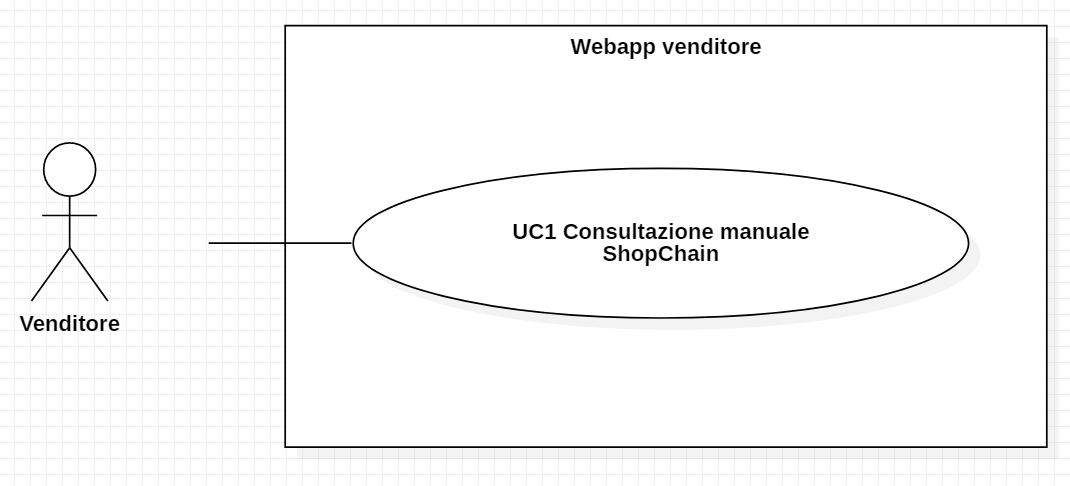
\includegraphics[width=0.7\textwidth]{UC_WAV1}

\paragraph{UC1 - Consultazione manuale ShopChain}\\
\textbf{Attori primari}: Venditore.\\
\textbf{Precondizioni}: Il venditore usa il servizio ShopChain e vorrebbe avere più informazioni sul suo utilizzo.\\
\textbf{Postcondizioni}: Il venditore consulta il manuale utente di ShopChain.\\
\textbf{Scenario principale}:\\
\begin{enumerate}
\item al venditore viene fornito il manuale utente già dall'acquisizione del prodotto ShopChain.
\item il venditore è libero di consultare il manuale in ogni momento.
\end{enumerate}

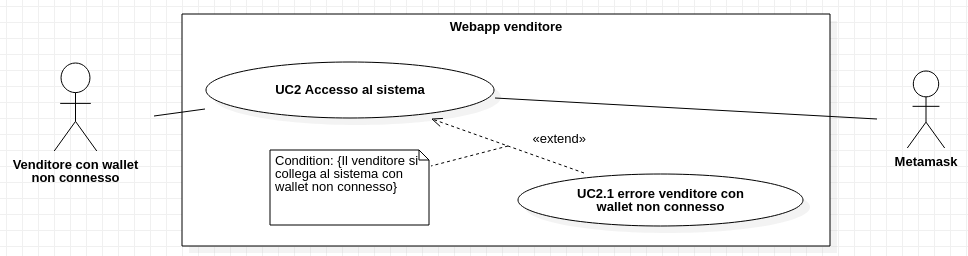
\includegraphics[width=0.9\textwidth]{UC_WAV2}

\paragraph{UC2 - Accesso al sistema (webapp venditore)}\\
\textbf{Attore primario}: Venditore con wallet non connesso.\\
\textbf{Attore secondario}: Metamask.\\
\textbf{Precondizioni}: Il venditore vuole accedere alla webapp.\\
\textbf{Postcondizioni}: Il venditore si è connesso alla webapp con Metamask.\\
\textbf{Scenario principale}:
Il venditore usando Metamask, si connette alla webapp con il proprio wallet.

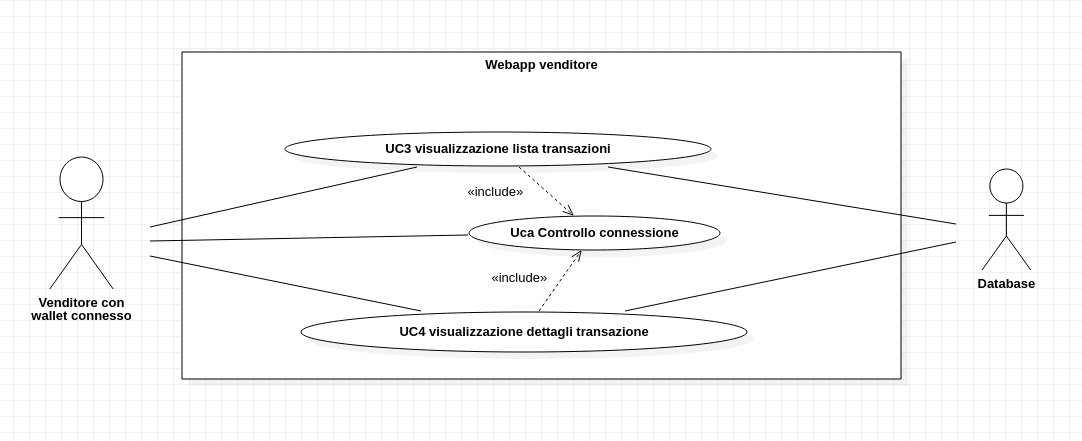
\includegraphics[width=0.9\textwidth]{UC_WAV3}

\paragraph{UC3 visualizzazione lista transazioni}\\
\textbf{Attore primario}: Venditore con wallet connesso. \\
\textbf{Attore secondario}: Database. \\
\textbf{Precondizioni}: Il venditore ha effettuato l'accesso al sistema.\\
\textbf{Postcondizioni}:  Il venditore vede la lista delle transazioni.\\
\textbf{Scenario principale}:
\begin{enumerate}
\item Il venditore vede la lista delle transazioni;
\item Il venditore può scegliere che tipo di transazioni vedere (tutte, completate, in attesa);
\item Il sistema mostra al venditore l'elenco delle transazioni richieste.
\end{enumerate}

\paragraph{UC4 - visualizzazione dettaglio transazione}\\
\textbf{Attore primario}: Venditore con wallet connesso.\\
\textbf{Attore secondario}: Database.\\
\textbf{Precondizioni}: Il venditore ha acceduto alla funzionalità di visualizzazione della lista delle transazioni.\\
\textbf{Postcondizioni}: Il venditore vede i dettagli di una singola transazione.\\
\textbf{Scenario principale}:
\begin{enumerate}
\item il venditore seleziona una delle transazioni dall'elenco;
\item il venditore visualizza i dettagli della singola transazione.
\end{enumerate}

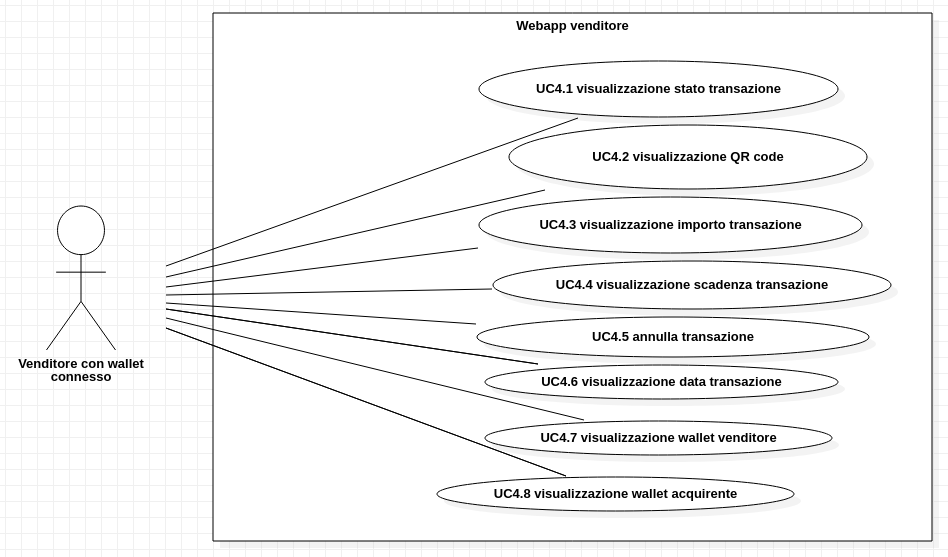
\includegraphics[width=0.9\textwidth]{UC_WAV4}

\paragraph{4.1 - Visualizzazione stato transazione}\\
\textbf{Attore primario}: Venditore con wallet connesso.\\
\textbf{Precondizioni}: Il venditore vuole visualizzare lo stato di una transazione.\\
\textbf{Postcondizioni}: Il venditore visualizza lo stato di una transazione.\\
\textbf{Scenario principale}: Viene visualizzato lo stato della transazione: in attesa oppure completata.\\

\paragraph{UC4.2 - Visualizzazione QR Code}\\
\textbf{Attore primario}: Venditore con wallet connesso.\\
\textbf{Precondizioni}: Il venditore vuole ottenere il QR Code di una transazione in attesa.\\
\textbf{Postcondizioni}: Il venditore è in possesso del QR Code da applicare sul pacco del prodotto.\\
\textbf{Scenario principale}:
\begin{enumerate}
\item viene visualizzato il QR Code della transazione in attesa selezionata;
\item il venditore può stampare il QR Code applicarlo sul pacco del prodotto.
\end{enumerate}

\paragraph{UC4.3 - Visualizzazione importo transazione}\\
\textbf{Attore primario}: Venditore con wallet connesso.\\
\textbf{Precondizioni}: Il venditore vuole visualizzare l'importo di una transazione.\\
\textbf{Postcondizioni}: Il venditore visualizza l'importo di una transazione.\\
\textbf{Scenario principale}: Viene visualizzato l'importo della transazione in dollari.\\

\paragraph{UC4.4 - Visualizzazione scadenza transazione}\\
\textbf{Attore primario}: Venditore  con wallet connesso.\\
\textbf{Precondizioni}: Il venditore vuole visualizzare la scadenza di una transazione in attesa.\\
\textbf{Postcondizioni}: Il venditore visualizza la scadenza di una transazione in attesa.\\
\textbf{Scenario principale}: Il venditore vede la data della scadenza di una transazione in attesa, oltre la quale l'acquirente riceverà indietro la valuta bloccata.\\

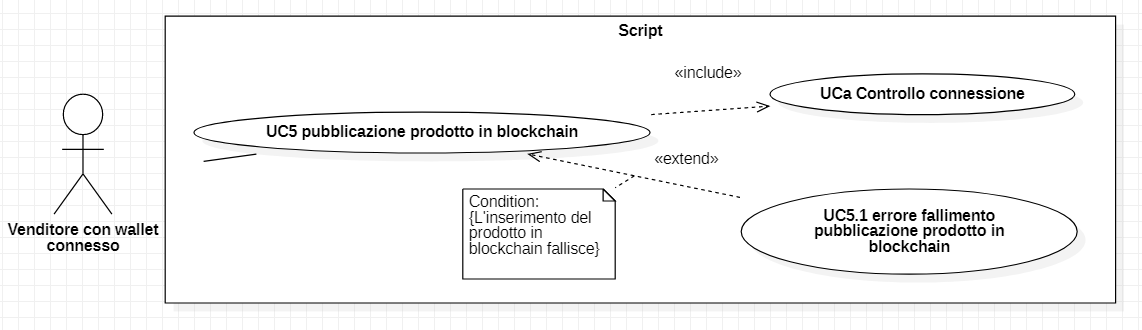
\includegraphics[width=0.9\textwidth]{UC_script}

\paragraph{UC5 - Pubblicazione prodotto in blockchain}\\
\textbf{Attore primario}: Venditore con wallet connesso.\\
\textbf{Precondizioni}: Il venditore ha integrato lo script nell'e-commerce e ha inserito un nuovo prodotto nell'e-commerce.\\
\textbf{Postcondizioni}: Il venditore ha pubblicato il nuovo prodotto in blockchain.\\
\textbf{Scenario principale}:
\begin{enumerate}
    \item il venditore inserisce un nuovo prodotto nell'e-commerce;
    \item tramite lo script il prodotto viene pubblicato in blockchain;
    \item il prodotto è pubblico in blockchain e utilizzabile per fare nuove transazioni.
\end{enumerate}
\textbf{Estensione}:
UC5.1 errore fallimento pubblicazione prodotto in blockchain:\\
lo script salva in un file di log il messaggio di errore.


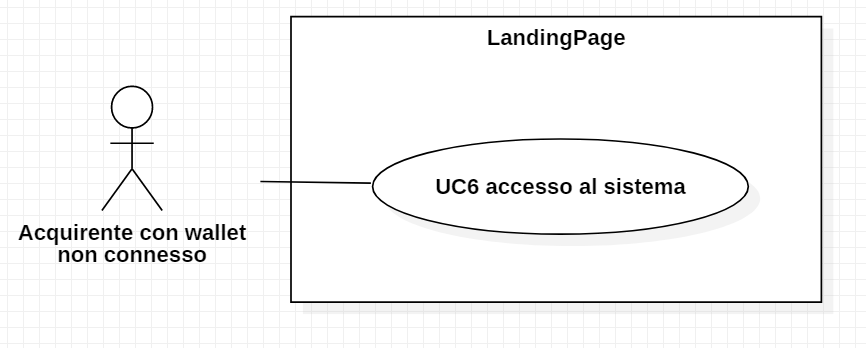
\includegraphics[width=0.9\textwidth]{UC_LP1}

\paragraph{UC6 - Accesso al sistema (landing page)}\\
\textbf{Attore primario}: Acquirente con wallet non connesso.\\
\textbf{Attore secondario}: Metamask.\\
\textbf{Precondizioni}: L'acquirente in landing page non è connesso con Metamask.\\
\textbf{Postcondizioni}: L'acquirente accede al sistema.\\
\textbf{Scenario principale}:
L'acquirente usando Metamask, si connette con il proprio wallet.

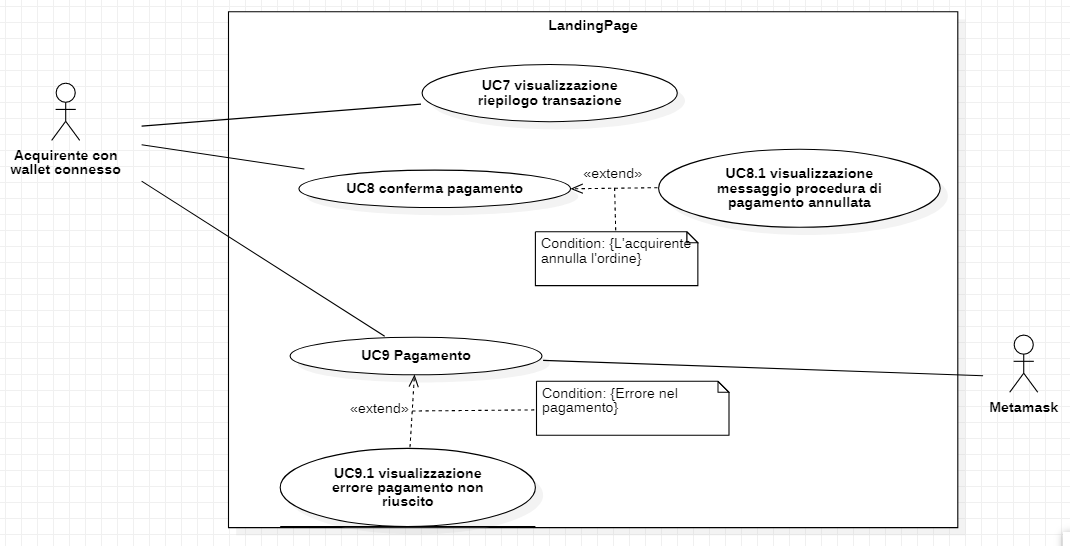
\includegraphics[width=0.9\textwidth]{UC_LP2}

\paragraph{UC7 - Visualizzazione riepilogo transazione}\\
\textbf{Attore primario}: Acquirente con wallet connesso.\\
\textbf{Precondizioni}: L'acquirente con wallet connesso vuole effettuare un acquisto usando ShopChain.\\
\textbf{Postcondizioni}: Il sistema mostra il riepilogo della transazione.\\
\textbf{Scenario principale}:
Viene mostrato all'acquirente il riepilogo della transazione con il prezzo in dollari da pagare.

\paragraph{UC8 - Conferma pagamento}\\
\textbf{Attore primario}: Acquirente con wallet connesso.\\
\textbf{Precondizioni}: L'acquirente sta effettuando un acquisto e il sistema mostra il riepilogo della transazione.\\
\textbf{Postcondizioni}: L'acquirente ha confermato il pagamento.\\
\textbf{Scenario principale}:
\begin{enumerate}
    \item il sistema mostra il riepilogo della transazione;
    \item l'acquirente conferma l'ordine.
\end{enumerate}
\textbf{Estensione}:
UC8.1 Visualizzazione messaggio procedura di pagamento annullata:
\begin{enumerate}
    \item visualizzazione messaggio procedura di pagamento annullata;
    \item cancellazione sessione di pagamento.
\end{enumerate}

\paragraph{UC9 - Pagamento}\\
\textbf{Attore primario}: Acquirente con wallet connesso.\\
\textbf{Attore secondario}: Metamask.\\
\textbf{Precondizioni}: L'acquirente ha confermato il pagamento.\\
\textbf{Postcondizioni}: Il pagamento è stato completato con successo.\\
\textbf{Scenario principale}:
\begin{enumerate}
    \item l'acquirente avvia la procedura di pagamento;
    \item l'acquirente effettua il pagamento tramite Metamask;
    \item l'ordine è stato pagato.
\end{enumerate}
\textbf{Estensioni}:
UC9.1 visualizzazione errore pagamento non riuscito:
\begin{enumerate}
    \item il pagamento non è stato completato con successo;
    \item cancellazione sessione di pagamento.
\end{enumerate}

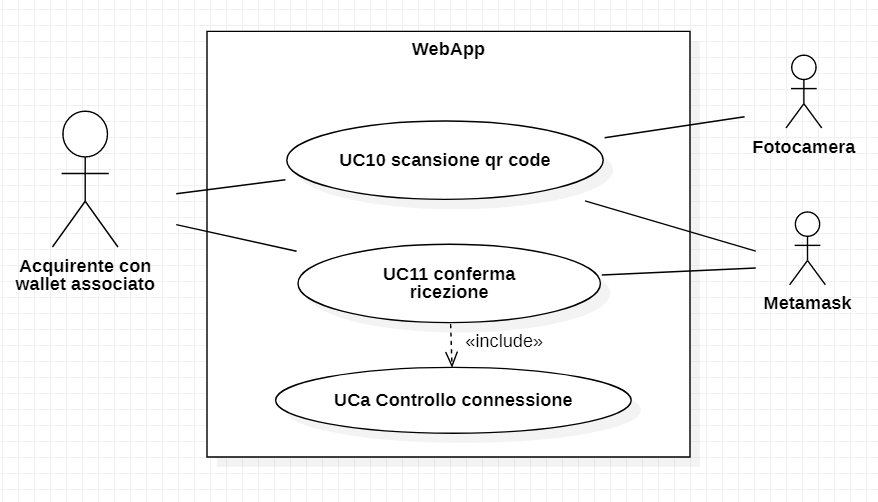
\includegraphics[width=0.9\textwidth]{UC_WAA1}

\paragraph{UC10 - Accesso al sistema (WebApp Acquirente)}\\
\textbf{Attore primario}: Acquirente con wallet non connesso.\\
\textbf{Attore secondario}: Metamask.\\
\textbf{Precondizioni}: L'acquirente nella webapp acquirente non è connesso con Metamask.\\
\textbf{Postcondizioni}: L'acquirente accede al sistema.\\
\textbf{Scenario principale}:
L'acquirente usando Metamask, si connette con il proprio wallet.

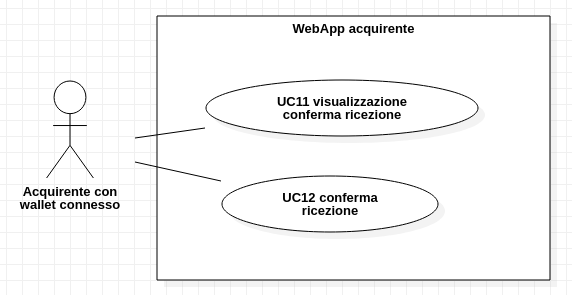
\includegraphics[width=0.9\textwidth]{UC_WAA2}

\paragraph{UC11 - Visualizzazione conferma ricezione}\\
\textbf{Attore primario}: Acquirente con wallet connesso.\\
\textbf{Precondizioni}: L'acquirente è connesso con Metamask ed è arrivato alla pagina di conferma ricezione scansionando il QR Code sul pacco del prodotto.\\
\textbf{Postcondizioni}: L'acquirente visualizza la pagina della transazione relativa al pacco appena ricevuto.\\
\textbf{Scenario principale}:
Vengono mostrati i dati relativi alla transazione e un pulsante per confermare la ricezione del pacco.

\paragraph{UC12 - Conferma ricezione}\\
\textbf{Attore primario}: Acquirente con wallet connesso.\\
\textbf{Precondizioni}: L'acquirente è connesso con Metamask alla pagina di conferma ricezione e conferma la ricezione del pacco.\\
\textbf{Postcondizioni}: L'acquirente ha confermato la ricezione del pacco, i fondi sono stati sbloccati.\\
\textbf{Scenario principale}:
\begin{enumerate}
    \item l'acquirente controlla sia tutto corretto e conferma la ricezione del pacco;
    \item il denaro viene sbloccato e mandato nel wallet del venditore.
\end{enumerate}
\textbf{Estensione}:
UC12.1 Errore wallet non corretto:
\begin{enumerate}
    \item Viene mostrato un messaggio di errore spiegando che il wallet con cui è connesso l'acquirente non è corretto.
    \item Si invita a cambiare wallet e riprovare.
\end{enumerate}

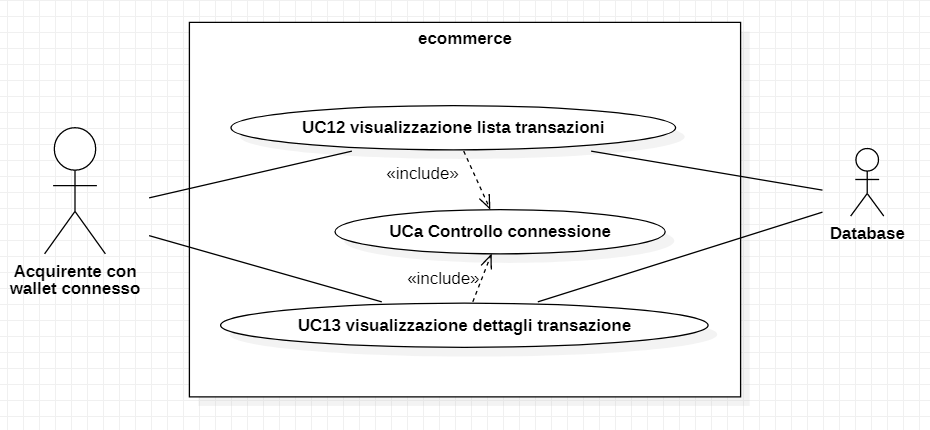
\includegraphics[width=0.9\textwidth]{UC_ECA1}

\paragraph{UC13 - Accesso al sistema (pagina lista transazioni acquirente in e-commerce)}\\
\textbf{Attore primario}: Acquirente con wallet non connesso.\\
\textbf{Attore secondario}: Metamask.\\
\textbf{Precondizioni}: L'acquirente, nella pagina con la sua lista delle transazioni in e-commerce, non è connesso con Metamask.\\
\textbf{Postcondizioni}: L'acquirente accede alla pagina con la sua lista delle transazioni in e-commerce.\\
\textbf{Scenario principale}:
L'acquirente usando Metamask, si connette con il proprio wallet.

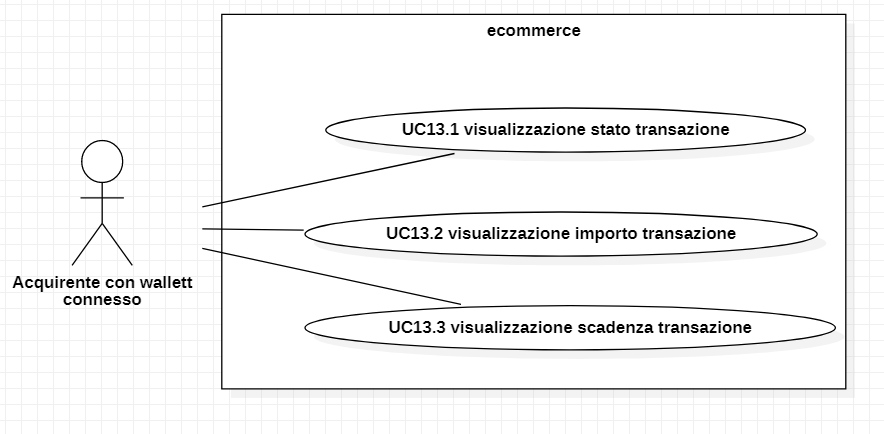
\includegraphics[width=0.9\textwidth]{UC_ECA2}

\paragraph{UC14 visualizzazione lista transazioni}\\
\textbf{Attore primario}: Acquirente con wallet connesso. \\
\textbf{Attore secondario}: Database. \\
\textbf{Precondizioni}: L'acquirente ha effettuato l'accesso al sistema.\\
\textbf{Postcondizioni}:  L'acquirente vede la lista delle transazioni.\\
\textbf{Scenario principale}:
\begin{enumerate}
\item L'acquirente vede la lista delle transazioni;
\item L'acquirente può scegliere che tipo di transazioni vedere (tutte, completate, in attesa);
\item Il sistema mostra all'acquirente l'elenco delle transazioni richieste.
\end{enumerate}

\paragraph{UC15 - visualizzazione dettaglio transazione}\\
\textbf{Attore primario}: Acquirente con wallet connesso.\\
\textbf{Attore secondario}: Database.\\
\textbf{Precondizioni}: L'acquirente ha acceduto alla funzionalità di visualizzazione della lista delle transazioni.\\
\textbf{Postcondizioni}: L'acquirente vede i dettagli di una singola transazione.\\
\textbf{Scenario principale}:
\begin{enumerate}
\item L'acquirente seleziona una delle transazioni dall'elenco;
\item L'acquirente visualizza i dettagli della singola transazione.
\end{enumerate}

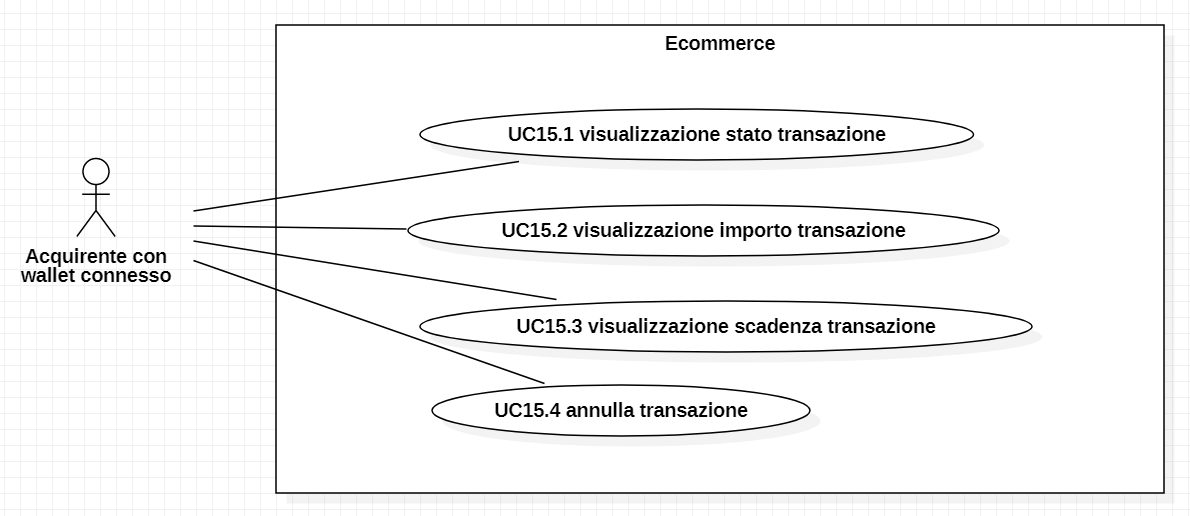
\includegraphics[width=0.9\textwidth]{UC_ECA3}

\paragraph{UC15.1 - Visualizzazione stato transazione}\\
\textbf{Attore primario}: Acquirente con wallet connesso.\\
\textbf{Precondizioni}: L'acquirente vuole visualizzare lo stato di una transazione.\\
\textbf{Postcondizioni}: L'acquirente visualizza lo stato di una transazione.\\
\textbf{Scenario principale}: Viene mostrato lo stato della transazione: in attesa o completata.\\

\paragraph{UC15.2 - Visualizzazione importo transazione}\\
\textbf{Attore primario}: Acquirente con wallet connesso.\\
\textbf{Precondizioni}: L'acquirente vuole visualizzare l'importo di una transazione.\\
\textbf{Postcondizioni}: L'acquirente visualizza l'importo di una transazione.\\
\textbf{Scenario principale}: Viene mostrato l'importo della transazione in dollari.\\

\paragraph{UC15.3 - Visualizzazione scadenza transazione}\\
\textbf{Attore primario}: Acquirente  con wallet connesso.\\
\textbf{Precondizioni}: L'acquirente vuole visualizzare la scadenza di una transazione in attesa.\\
\textbf{Postcondizioni}: L'acquirente visualizza la scadenza di una transazione in attesa.\\
\textbf{Scenario principale}: Viene visualizzata la data della scadenza di una transazione in attesa, oltre la quale l'acquirente riceverà indietro la valuta bloccata.\\

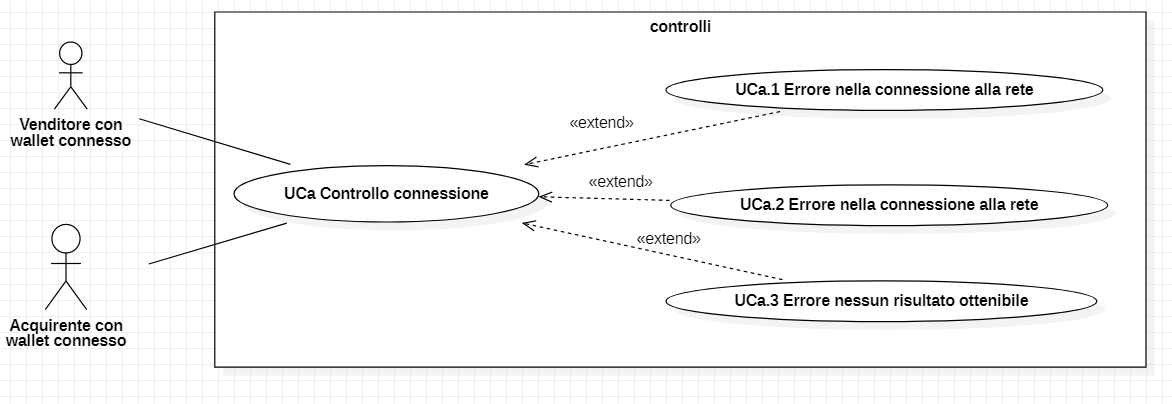
\includegraphics[width=0.9\textwidth]{UC_controlli}

\paragraph{UCa Controllo connessione}\\
\textbf{Attori primari}: Venditore con wallet connesso, Acquirente con wallet connesso. \\
\textbf{Precondizioni}: Il sistema vuole interagire con la blockchain.\\
\textbf{Postcondizioni}:  Il sitema può interagire con la blockchain senza problemi.\\
\textbf{Scenario principale}:
Vengono fatti una serie di controlli per la corretta interazione con la blockchain.\\
\textbf{Estensioni}:
\begin{enumerate}
    \item UCa.1 Errore nella connessione alla rete:\\
        Il venditore o l'acquirente è connesso alla rete sbagliata
    \item UCa.2 Errore transazione non inviata:\\
        La transazione non è stata inviata correttamente.
    \item UCa.3 Errore nessun risultato ottenibile:\\
        La transazione è stata correttamente inviata, ma non è stato ottenuto nessun risultato.
\end{enumerate}

\section{Requisiti}
Ogni requisito è indentificato da un codice univoco composto da: R(per requisito)+F/N(per la tipologia: funzionale, non funzionale)+O/D/F(per la rilevanza: obbligatorio, desiderabile, facoltativo)+x(un numero univoco a due cifre).
\subsection{Requisiti funzionali}
 
 \setlength\tabcolsep{4pt}
\begin{longtable}{|c|p{5cm}|c|c|}
\hline
 \multicolumn{4}{| c |}{Requisiti funzionali}\\
 \hline
 Codice & Descrizione & rilevanza & fonti\\
 \hline
 \endfirsthead

 \hline
 \multicolumn{4}{| c |}{Requisiti funzionali}\\
 \hline
 Codice & Descrizione & Rilevanza & Fonti\\
 \hline
 \endhead
% WEBAPP VENDITORE
\hline
RFO01 & Per accedere alla webapp venditore il venditore con wallet non connesso deve connettere il proprio wallet tramite Metamask. & Obbligatorio & UC2 \\
\hline
RFO02 & Un venditore con wallet non connesso non può accedere alla webapp venditore. & Obbligatorio & Capitolato, decisione interna \\
\hline
RFO03 & Il venditore deve poter visualizzare la lista delle transazioni nella webapp venditore. & Obbligatorio & UC3 \\ 
\hline
RFO04 & Il venditore deve poter visualizzare nella webapp venditore, per ogni transazione, il suo stato (attesa o completata). & Obbligatorio & UC4.1 \\ 
\hline
RFO05 & Il venditore deve poter visualizzare nella webapp venditore, per ogni transazione, il QR Code da applicare sul pacco. & Obbligatorio & UC4.2 \\ 
\hline
RFO06 & Il venditore deve poter visualizzare nella webapp venditore, per ogni transazione, l'importo in dollari. & Obbligatorio & UC4.3 \\ 
\hline
RFO07 & Il venditore deve poter visualizzare nella webapp venditore, per ogni transazione, la scadenza della transazione. & Obbligatorio & UC4.4 \\ 
\hline
RFO08 & L'acquirente deve ricevere indietro la valuta bloccata con cui ha pagato per la transazione, quando la transazione scade. & Obbligatorio & Decisione interna, UC4.4 \\ 
\hline
% SCRIPT
RFO09 & Il prodotto deve essere pubblicato automaticamente in blockchain, quando il venditore inserisce un nuovo prodotto nell'e-commerce, grazie al nostro script incluso dal venditore nel suo e-commerce. & Obbligatorio & UC5 \\ 
\hline
RFO10 & Il nostro script deve salvare un messaggio di errore in un file di log, se la pubblicazione del prodotto in blockchain dall'e-commerce (grazie allo script) fallisce. & Obbligatorio & UC5.1 \\ 
\hline
% LANDING PAGE
RFO11 & Per accedere alla landing page l'acquirente con wallet non connesso deve connettere il proprio wallet tramite Metamask. & Obbligatorio & UC6, UC15 \\
\hline
RFO12 & Un acquirente con wallet non connesso non può accedere alla landing page. & Obbligatorio & Capitolato, decisione interna \\
\hline
RFO13 & L'acquirente con wallet connesso deve vedere il prezzo da pagare in dollari nella landing page. & Obbligatorio & UC7 \\
\hline
RFO14 & L'acquirente con wallet connesso poter confermare il pagamento nella landing page. & Obbligatorio & UC8 \\
\hline
RFO15 & Il sistema deve mostrare un messaggio "ordine annullato" se l'acquirente con wallet connesso annulla il pagamento sulla landing page. & Obbligatorio & UC8.1 \\
\hline
RFO16 & Il sistema deve cancellare la sessione di pagamento se l'acquirente con wallet connesso annulla il pagamento sulla landing page. & Obbligatorio & UC8.1 \\
\hline
RFO17 & L'acquirente con wallet connesso deve essere indirizzato automaticamente su Metamask per completare il pagamento, quando conferma il pagamento sulla landing page. & Obbligatorio & UC9 \\
\hline
RFO18 & Il sistema deve cancellare la sessione di pagamento, se il pagamento non va a buon fine quando l'acquirente con wallet connesso effettua il pagamento tramite Metamask. & Obbligatorio & UC9.1 \\
\hline
% WEBAPP ACQUIRENTE
RFO19 & Per accedere alla webapp acquirente, l'acquirente con wallet non connesso deve connettere il proprio wallet tramite Metamask. & Obbligatorio & UC10 \\
\hline
RFO20 & Un acquirente con wallet non connesso non può accedere alla webapp acquirente. & Obbligatorio & Capitolato, decisione interna \\
\hline
RFO21 & L'acquirente con wallet connesso deve poter vedere il prezzo in dollari e in cryptovaluta nella webapp acquirente, dopo essere atterrato nella webapp acquirente scansionando il QR Code sul pacco. & Obbligatorio & UC11 \\
\hline
RFO22 & L'acquirente con wallet connesso deve poter confermare la ricezione del pacco nella webapp acquirente, dopo essere atterrato nella webapp acquirente scansionando il QR Code sul pacco. & Obbligatorio & UC12 \\
\hline
RFO23 & Il sistema deve mostrare un messaggio di errore "wallet non corretto" nella webapp acquirente, nel caso in cui dopo aver confermato la ricezione del pacco nella webapp acquirente, il sistema rileva che il wallet non corrisponde a quello che ha effettuato la transizione. & Obbligatorio & UC12.1 \\
\hline
% ECOMMERCE
RFO24 & Per accedere alla pagina con la sua lista delle transazioni in e-commerce, l'acquirente con wallet non connesso deve connettere il proprio wallet tramite Metamask. & Obbligatorio & UC13 \\
\hline
RFO25 & Un acquirente con wallet non connesso non può accedere alla pagina con la sua lista delle transazioni in e-commerce. & Obbligatorio & Capitolato, decisione interna \\
\hline
RFO26 & L'acquirente con wallet connesso deve poter visualizzare la lista delle sue transazioni in una pagina apposita, dedicata all'e-commerce. & Obbligatorio & UC14 \\
\hline
RFO27 & L'acquirente con wallet connesso deve poter visualizzare lo stato di ogni sua transazione (attesa o completata) in una pagina apposita, dedicata all'e-commerce. & Obbligatorio & UC15.1 \\
\hline
RFO28 & L'acquirente con wallet connesso deve poter visualizzare l'importo di ogni sua transazione in una pagina apposita, dedicata all'e-commerce. & Obbligatorio & UC15.2 \\
\hline
RFO29 & L'acquirente con wallet connesso deve poter visualizzare l'importo in dollari di ogni sua transazione in una pagina apposita, dedicata all'e-commerce. & Obbligatorio & UC15.2 \\
\hline
RFO30 & L'acquirente con wallet connesso deve poter visualizzare la scadenza di ogni sua transazione in una pagina apposita, dedicata all'e-commerce. & Obbligatorio & UC15.3 \\
\hline
% CONTROLLI
RFO31 & Il sistema deve mostrare un messaggio di errore "Errore nella connessione alla rete" se l'utente(acquirente o venditore) è connesso alla rete sbagliata. & Obbligatorio & UCa.1 \\
\hline
RFO32 & Il sistema deve mostrare un messaggio di errore "Errore transazione non inviata" se la transazione non è stata inviata in maniera corretta. & Obbligatorio & UCa.2 \\
\hline
RFO33 & Il sistema deve mostrare un messaggio di errore "Errore nessun risultato ottenibile" se la transazione è stata inviata in maniera corretta ma non è stata ottenuto alcun risultato di risposta. & Obbligatorio & UCa.3 \\
\hline

\end{longtable}
\pagebreak

\setlength\tabcolsep{4pt}
\begin{longtable}{|c|p{5cm}|c|c|}
\hline
 \multicolumn{4}{| c |}{Requisiti non funzionali}\\
 \hline
 Codice & Descrizione & rilevanza & fonti\\
 \hline
 \endfirsthead

 \hline
 \multicolumn{4}{| c |}{Requisiti non funzionali}\\
 \hline
 Codice & Descrizione & Rilevanza & Fonti\\
 \hline
 \endhead

\hline
RNO01 & Utilizzo di blockchain pubblica. & Obbligatorio & Capitolato, decisione interna \\
\hline
RND02 & Utilizzo di database PostgreSQL. & Desiderabile & Capitolato \\
\hline
RNO03 & Il venditore deve disporre di un manuale utente per l'utilizzo del sistema. & Obbligatorio &  UC1, decisione interna\\
\hline
RNO04 & Test che dimostrino il corretto funzionamento dei servizi e delle funzionalità previste,
con una copertura minima dell’ 80\% correlata di report. & Obbligatorio & Capitolato\\
\hline
RNO05 & Documentazione su scelte implementative e progettuali effettuate, le relative motivazioni, i problemi aperti e le eventuali soluzioni proposte da esplorare. & Obbligatorio & Capitolato\\
\hline
RNO06 & Deve essere reso disponibile uno script python scaricabile dai venditori da integrare nel loro e-commerce per la pubblicazione automatica dei nuovi prodotti in BlockChain. & Obbligatorio & UC5, decisione interna\\
\hline

\end{longtable}



\end{document}